%%
%% Copyright 2007, 2008, 2009 Elsevier Ltd
%%
%% This file is part of the 'Elsarticle Bundle'.
%% ---------------------------------------------
%%
%% It may be distributed under the conditions of the LaTeX Project Public
%% License, either version 1.2 of this license or (at your option) any
%% later version.  The latest version of this license is in
%%    http://www.latex-project.org/lppl.txt
%% and version 1.2 or later is part of all distributions of LaTeX
%% version 1999/12/01 or later.
%%
%% The list of all files belonging to the 'Elsarticle Bundle' is
%% given in the file `manifest.txt'.
%%
%% Template article for Elsevier's document class `elsarticle'
%% with harvard style bibliographic references
%% SP 2008/03/01

\documentclass[final,3p,times,twocolumn]{elsarticle}

%% Use the option review to obtain double line spacing
%% \documentclass[authoryear,preprint,review,12pt]{elsarticle}

%% Use the options 1p,twocolumn; 3p; 3p,twocolumn; 5p; or 5p,twocolumn
%% for a journal layout:
%% \documentclass[final,1p,times]{elsarticle}
%% \documentclass[final,1p,times,twocolumn]{elsarticle}
%% \documentclass[final,3p,times]{elsarticle}
%% \documentclass[final,3p,times,twocolumn]{elsarticle}
%% \documentclass[final,5p,times]{elsarticle}
%% \documentclass[final,5p,times,twocolumn]{elsarticle}

%% For including figures, graphicx.sty has been loaded in
%% elsarticle.cls. If you prefer to use the old commands
%% please give \usepackage{epsfig}

%% The amssymb package provides various useful mathematical symbols
\usepackage{amssymb}
\usepackage{epstopdf}
\usepackage{hyperref}
\usepackage{color}

%% The amsthm package provides extended theorem environments
%% \usepackage{amsthm}

%% The lineno packages adds line numbers. Start line numbering with
%% \begin{linenumbers}, end it with \end{linenumbers}. Or switch it on
%% for the whole article with \linenumbers.
%% \usepackage{lineno}

\journal{Applied Acoustics}

\newcommand{\ml}[1]{\textcolor{blue}{ Mathieu: #1}}


\begin{document}

\begin{frontmatter}

%% Title, authors and addresses

%% use the tnoteref command within \title for footnotes;
%% use the tnotetext command for theassociated footnote;
%% use the fnref command within \author or \address for footnotes;
%% use the fntext command for theassociated footnote;
%% use the corref command within \author for corresponding author footnotes;
%% use the cortext command for theassociated footnote;
%% use the ead command for the email address,
%% and the form \ead[url] for the home page:
%% \title{Title\tnoteref{label1}}
%% \tnotetext[label1]{}
%% \author{Name\corref{cor1}\fnref{label2}}
%% \ead{email address}
%% \ead[url]{home page}
%% \fntext[label2]{}
%% \cortext[cor1]{}
%% \address{Address\fnref{label3}}
%% \fntext[label3]{}


\title{An efficient audio coding scheme for large scale acoustic monitoring}

%% use optional labels to link authors explicitly to addresses:
%% \author[label1,label2]{}
%% \address[label1]{}
%% \address[label2]{}

\author{Felix Gontier, Mathieu Lagrange, Arnaud Can, Catherine Lavandier}

\address{felix.gontier@reseau.eseo.fr\\mathieu.lagrange@cnrs.fr}

\begin{abstract}
%% Text of abstract
The advent of low cost acoustic sensors together with the need to better monitor and comprehend the acoustic environment of urban and wilderness areas give rise to the deployment of experimental sensor networks such as the sonyc (wp.nyu.edu/sonyc) and cense (cense.ifsttar.fr) projects.

Together with the estimation of acoustic indicators (LAeq, ...), one important aspect of those networks is their ability to detect the presence of sound sources of interest ( bird calls, sirens, explosion, ...) in order to better assess soundscapes. This detection step can be operated online (on the sensors) or offline (on the data servers).

The former is efficient in terms of data storage as only the detection events are transmitted. Though, it requires the availability of computing resources on the sensors in order to perform the detection step, and the detection is done once and cannot be recomputed.

The latter scheme has several benefits. First, the sensor is much simpler and can thus be autonomous in terms of energy, easing the deployment of the network. Second, it allows researchers to gather large amount of data that can be post processed and studied further offline. Data can be re analysed following newer classification schemes or using new indicators.

But, for transmission from the sensors to the storage unit, the data needs to be encoded in an efficient way. Also, as the data is transmitted using the network and stored, one must ensure that the intelligibility of potential speech utterances is lost during the coding process, in order to ensure the privacy of the citizens.

The coding scheme described in this paper has the following features. It is of low bitrate but still allows the computation of most of the standard acoustics indicators with high precision. As far as acoustic event detection is concerned, we report equivalent performance of several state of the art classification schemes from features computed using raw audio data and encoded data. Finally, according to preliminary perceptual evaluation, the proposed coding scheme very strongly degrades the intelligibility, thus ensuring citizen privacy.

In order to promote reproducible research, the coder as well as the experiments needed to generate the figures will be made available to the community.



\end{abstract}

\begin{keyword}
%% keywords here, in the form: keyword \sep keyword

%% PACS codes here, in the form: \PACS code \sep code

%% MSC codes here, in the form: \MSC code \sep code
%% or \MSC[2008] code \sep code (2000 is the default)

\end{keyword}

\end{frontmatter}

%% \linenumbers
\clearpage
%% main text
\section{Introduction}
%\label{}

\section{Background}

The present work is constrained to allow both acoustic monitoring and sound event recognition in urban soundscapes. Here we briefly review state-of-the-art methods in both subjects to guide our choices.

\subsection{Acoustic monitoring}

The considered sensor network primarily aims at monitoring urban soundscapes, that is, continously assessing their content and impact on the population. This is typically enabled by measuring energetic acoustic indicators such as the equivalent sound pressure level $L_{eq}$ in dB SPL or its A-weighted equivalent $L_{Aeq}$ in dBA. However, while these indicators have proven to correlate well with perceptual evaluations for negative impact sound environments \cite{gozalo2015}, they fail to fully describe soundscapes \cite{rychtarikova2013}. Many other variables can be derived to better account for previously implicit properties \cite{can2016} including percentile values or time evolution. Studies have been conducted to select relevant subsets of descriptors in sound environment characterization \cite{can2015, brocolini2013, nilsson2007}.\\

All the mentionned indicators are measured at periods ranging from 0.125~ms or 1~s (resp. fast and slow) to longer periods of several minutes. Therefore, sound frequency information remains unused despite being closely related with subjective evaluations \cite{ishiyama2000}. A simple solution is the calculation of energetic indicators for the 31 third-octave bands within the human audition range 20~Hz - 20~kHz.\\

This measurement appears well-suited for this work's purpose: in addition to being an efficient descriptor \cite{torija2013}, it allows for the computation of most cited indicators while representing reasonably small, fixed amounts of data to be transmitted.

\subsection{Event detection}

Another major interest of this work is sound event recognition. This problem has been the subject of extensive research in the past on speech \cite{anusuya2009}, music \cite{tzanetakis2002}, and lately more complex scenes in which the current work falls. Studied classification methods are diverse, ranging from time-dependant modeling with HMMs \cite{ntalampiras2014} to "bag-of-frames" approaches \cite{aucouturier2007, foggia2015}. Common architectures include learning-based classifiers such as support vector machines (SVM) \cite{kumar2016}, gaussian mixture models (GMM) \cite{radhakrishnan2005} or neural networks \cite{salamon2017, piczak2015}. However, the selection of relevant features is still an open debate. The most used are certainly spectral \cite{khunarsal2013} or cepstral \cite{couvreur2004} representations of the signal. Among them, mel spectrograms and their cepstral-domain derivation, the mel-frequency cepstrum coefficients (MFCC), are the most recurrent. These representations effectively try to model the human cochlear response to sounds by grouping frequency components around critical bands in a logarithmic scale, thus bearing important physical significance. They may also be exploited together with features computed in other domains to better model signal properties. For instance, \cite{cai2006} adds spectral features related to harmonicity and salient frequencies, and \cite{chu2009} uses a matching pursuit (MP) algorithm to deduce time-domaid features. Another promising solution is feature engineering via unsupervised learning, which \cite{salamon2015-2} implements with a k-means clustering technique. Alternative data representations such as the scattering transform \cite{bauge2013} show good results in environmental sound classification tasks \cite{salamon2015}.\\
A more detailed review of used methods is available in \cite{chachada2013}.

\section{Encoding scheme}

The technical constraints of size inherent to the studied setup make it impossible to transmit raw audio recordings. Following the considerations briefly exposed in the previous section, we conclude that third-octave bands are a reasonable choice. As mentionned, they provide advantages in both acoustic monitoring and data volume per measurement period. The physical content is also close to that of mel spectrograms, being just another filterbank transform with logarithmic frequency scaling.\\

A common way to implement third-octave analysis is to first design the highest octave three filters, and use them on progressively time-decimated versions of the input signal \cite{davis1986}. In practice, however, this technique presents multiple issues. \cite{antoni2010} presents an alternative analysis method based on direct frequency weighting. The weights matrix design procedure complies with both ANSI S1.1-1986 and IEC 61260-1:2014 standards. It also respects the partition of unity principle over all frequency bins in the relevant range. Resulting filters for different parameter $l$ values are compared with Couvreur's implementation \cite{couvreur} of the time-domain filtering, as shown in Figure~\ref{fig:freq_filt}. The major difference is that gains at cutoff frequencies are fixed at the optimal -3dB by design.\\

\begin{figure}[htbp]
	\centering
		\includegraphics[width=\columnwidth]{tob_imp.eps}
	\caption{Comparison of Couvreur's and Antoni's implementations of third-octave filters. Frequency-weighting allows for arbitrary transfer functions and thus more accurate gains as standards impose.}
	\label{fig:freq_filt}
\end{figure}

The first step is to represent the signal in the frequency domain using a short-term Fourier transform (STFT). The continuously sampled audio is segmented into 125~ms frames to provide "fast" acoustic measurements. The data is zero-passed to the next power of two to allow best fft performances. No overlap is used as it doubles both computational and memory costs and is not required for our application. A rectangular window is applied to ensure energy conservation in a given analysis frame. The phase is unimportant to third-octave analysis, thus it is discarded. Similarly, negative frequency components contain the same information as positive ones because the base signal is real. We then compute third-octave bands from the squared spectral magnitude by matrix multiplication with the frequency weights proposed in \cite{antoni2010} for $l = 2$\footnote{When implementing said method, we found that squaring the $\phi_l(p), l \geq 1$ intermediate function (p. 887) was the correct approach to meet cutoff frequencies requirements, and we believe this was the author's original intention.}. We include analysis for bands $i$ from -17 to 13, ie. center frequencies $f_i$ ranging from $20~Hz$ to $20~kHz$ with $f_0 = 1~kHz$. This means the main representation is composed of 31 values sampled every 125~ms.\\

Alternatively, we also implement the mel filterbank for testing purposes. Mel spectrograms can be used as a baseline method to evaluate the relative performance of third-octave bands in sound event recognition. Furthermore, this representation is not bound by constraints such as conservation of energy, specific framing parameters or fixed resolution. It offers a more flexible tool to study intelligibility alteration and coder performance, both of which we take interest in. Mel spectrograms are computed with the \textit{rastamat} library \cite{ellis2005}. STFT analysis frames are obtained by applying a Hann window on 23.2~ms of signal with 50\% (11.6~ms) overlap to allow for efficient phase recovery in further tests.

\subsection{Data Encoding}

A Huffman coding scheme \cite{huffman1952} is then used to further reduce data dimensionality. As in most entropy coding algorithms, the efficiency of this technique depends on two important factors. A reduced amount of symbols in the dictionnary yields smaller code size on lower probability symbols. Lower data entropy, ie. lower average information content of the signal distribution, also increases performance. The first is generally obtained by applying a quantization process to the signal, whereas the second is directly linked with the probability density function (PDF) of these symbols. It is defined as $H = -\sum\limits_i p_ilog_n(p_i)$, where $p_i$ is the probability of appearance of a given symbol and $n$ the numerical base in which information is represented. As such, entropy decreases when very few symbols have a very high probability of appearance and is maximum for a uniform distribution. Considering an estimated PDF for our data as shown in Figure~\ref{fig:pdf}a, immediately applying a linear quantization clearly results in most of the information being lost. We therefore spread the PDF by taking the logarithm of the representation. A linear quantization is then applied with $2^{q-1}-1$ output values to obtain Figure~\ref{fig:pdf}b. Finally, we use a $\Delta$-encoding algorithm along the time dimension to reduce redundancies. This also effectively concentrates higher probabilities on symbols around zero (Figure~\ref{fig:pdf}c). This yields a higher amount of symbols at $2^q-1$ but a nevertheless smaller entropy. In the example shown here, the former is $H_{log} = 6.24~sh$ and the latter $H_{\Delta} = 3.54~sh$. Huffman encoding is then computed with either a frame-specific symbol-code dictionnary or a constant one generated from an entire dataset. A comparison of both methods is shown in Figure~\ref{fig:dict_comp}. For most short texture frame durations, we found the local Huffman algorithm to be much faster. In fact, encoding complexity is function of the amount of dictionnary elements. If it is specific to a given data packet, then it does not need to contain every possible value. This gain seem to outweight the additional complexity induced by the tree generation algorithm. Alternatively, short texture frames or single analysis windows can be encoded using one general dictionnary to improve bitrate. This choice depends on which of the size and complexity parameters must be reduced most.\\

\begin{figure}[htbp]
	\centering
		\includegraphics[width=0.5\textwidth]{pdf.eps}
	\caption{Example of estimated probability density functions of the data throughout the encoding step. (left) Unchanged output of the representation step, concentrated towards very low values. (middle) PDF "flattening" effect induced by logarithm application. Here values are mapped to the range $[0, 2^7-1]$ and rounded to perform quantization. (right) Output of the $\Delta$ compression, with desirable probabilities as the input to a Huffman algorithm.}
	\label{fig:pdf}
\end{figure}

\begin{figure}[htbp]
	\centering
		\includegraphics[width=\columnwidth]{dict_comp.eps}
	\caption{Performance comparison of locally and globally generated Huffman dictionnaries. (top) The mean execution time ratio favors the use of frame-specific dictionnaries for tested texture frame lengths. (bottom) The mean output bitrate is close for both algorithms, showing that the necessity of sending symbol-code pairs mostly compensates for their optimality.}
	\label{fig:dict_comp}
\end{figure}

The decoding process is quite straightforward, as both Huffman and $\Delta$ compression are lossless and directly reversible.

The entire coder scheme is summarized in Figure~\ref{fig:scheme}.

\begin{figure*}[htbp]
	\centering
		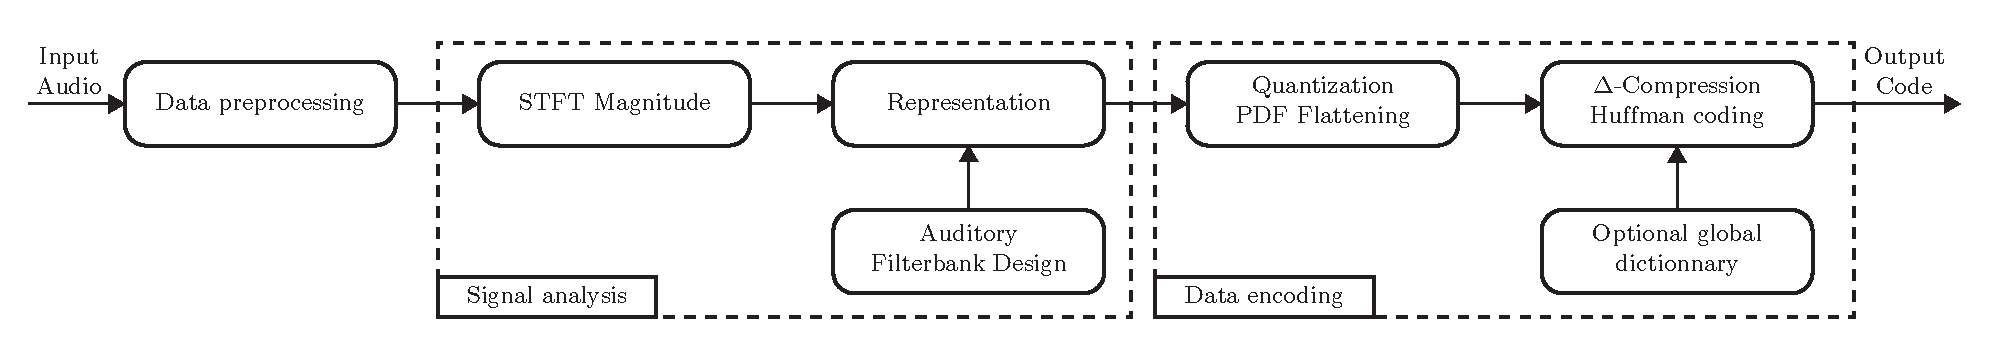
\includegraphics[width=1\textwidth]{scheme.pdf}
	\caption{Overview of the coder process.}
	\label{fig:scheme}
\end{figure*}

\section{Evaluation}
A set of metrics is computed to assess the efficiency of the proposed coder scheme and determine the impact of the algorithm's parameters, which are as follow: the desired word size prior to Huffman encoding, set by quantization for both signal representation choices, and only for Mel bands the number of coefficients between 10 and 40. We also study the effect of time averaging analysis frames: to force a fixed amount of frames per second lesser than the average speech rate in phonemes per second is a possible way to alter intelligibility at the cost of temporal information resolution.

\subsection{Efficiency}

The coder's output bitrate as well as additional measurement error is computed for both data representations, it is expressed in dB and compared to the IEC 61672-1:2013 standard on sound level meter tolerance. This is to verify that the quantization step yields a maximum absolute error inferior to the precision of the recording device. To provide relevant statistics, these quantities are estimated for a total of 53 10-minutes texture frames.

\subsection{Event recognition}

The UrbanSound8k dataset\cite{salamon2014} features about 9 hours of urban environmental sounds recordings separated in 8732 wave files ranging from 1 to 4 seconds each. The recordings are labeled in 10 classes (air conditioner, car horn, children playing, dog bark, drilling, enginge idling, gun shot, jackhammer, siren, street music), and distributed in 10 independant folds. A method and baseline results are also provided for the classification task. It is used in all the following experiments with the exception of intelligibility computation for which a small dataset of high-quality voice recordings is preferred. Audio files are resampled 44.1 samples per second, normalized and reduced to a single channel.\\

We first evaluate the global loss of information by implementing the four classification models proposed in \cite{salamon2014}: a support vector machine with a radial basis function kernel, a random forest classifier with 500 trees, a decision tree and a k-nearest neighbors classifier with $k = 5$. Values for the SVM parameter $C$ and RBF kernel variance $\sigma^2$ are found with a grid search. We apply a discrete cosine transform to the critical band signal representation to obtain cepstra (known as Mel Frequency Cepstrum Coefficients or MFCC in the first case) of which we conserve the 25 first coefficients, and summarize along time with the mean, variance, skewness, kurtosis, minimum, maximum, median, derivative mean and variance, second order derivative mean and variance. The feature vector is thus comprised of 275 values to reproduce available results and compare with our own. Models are trained for each setup using the 10-fold method, that is, every combination of testing one fold on models trained with the other nine.

\subsection{Inintelligibility}

Intelligibility in decoded and reconstructed audio is also one of the main concerns of this study. We conduct preliminary perceptive tests to ensure that a clean speech recording is made unintelligible, implying the same results in usually noisier urban soundscapes. We also provide the computation of two objective metrics: the Coherence Speech Intelligibility Index\cite{kates2005} (CSII) and frequency-eighted segmental SNR\cite{hu2008} (fwSNRseg) by comparing original unaltered samples and recovered audio. These two indicators have been shown to correlate well with perceptual tests\cite{ma2009}, although results are only available for lesser degradations and distortions.\\

These metrics require a recovery of the time-domain signal. We must first recover a linearly-scaled spectrogram from the band-focused representations. This can be achieved by multiplying by the scaled transpose of the forward transformation matrix. A loss of resolution increasing with frequency is induced due to the shape of the transformation, as illustrated by Figure~\ref{fig:freq}. Signal phase is approximated by either white noise spectrogram scaling or a Griffin\& Lim algorithm \cite{griffin1984}, and the signal is retrieved using overlap-add. When using overlap while computing third-octave bands, one can also avoid framing effects produced by rectangular windowing by convoluting the signal with another windowing function prior to inverse-STFT computation.\\

\begin{figure}[htbp]
	\centering
		\includegraphics[width=\columnwidth]{freq.png}
	\caption{Third-octave bands analysis and approximate inverse transformation effects on energy location. This process yields an important and heterogeneous loss in resolution, particularly at higher frequency points.}
	\label{fig:freq}
\end{figure}



\section{Results}

\section{Conclusion}

\clearpage
%% The Appendices part is started with the command \appendix;
%% appendix sections are then done as normal sections
%% \appendix

%% \section{}
%% \label{}

%% If you have bibdatabase file and want bibtex to generate the
%% bibitems, please use
%%
%%  \bibliographystyle{elsarticle-harv}
%%  \bibliography{<your bibdatabase>}

%% else use the following coding to input the bibitems directly in the
%% TeX file.
\section{References}
\begin{thebibliography}{09}






\bibitem{gozalo2015}
Rey Gozalo, G. and Trujillo Carmona, J. and Barrigon Morillas, J.M. and Gomez Escobar, V. (2015). Relationship between objective acoustic indices and subjective assessments for the quality of soundscapes. \textit{Applied Acoustics}, 97, pp. 1-10

\bibitem{rychtarikova2013}
Rychtarikova, M. and Vermeir, G. (2013). Soundscape categorization on the basis of objective acoustical parameters. \textit{Applied Acoustics}, 74(2), pp. 240-247

\bibitem{can2016}
Can, A. and Aumond, P. and Michel, S. and De Coensel, B. and Ribeiro, C. and Botteldooren, D. and Lavandier, C. (2016). Comparison of noise indicators in an urban context. In: \textit{Proceedings of the 45th International Congress and Exposition on Noise Control Engineering}, pp. 5678-5686

\bibitem{can2015}
Can, A. and Gauvreau, B. (2015). Describing and classifying urban sound environments with a relevant set of physical indicators. \textit{J. Ac. Soc. Am.}, 137(1), pp. 208-218

\bibitem{brocolini2013}
Brocolini, L. and Lavandier, C. and Quoy, M. and Ribeiro, C. (2013). Measurements of acoustic environments for urban soundscapes: Choice of homogeneous periods, optimization of durations, and selection of indicators. \textit{J. Ac. Soc. Am.}, 134(1), pp. 813-821

\bibitem{nilsson2007}
Nilsson, M. and Botteldooren, D. and De Coensel, B. (2007). Acoustic indicators of soundscape quality and noise annoyance in outdoor urban areas. In: \textit{Proceedings of the 19th International Congress on Acoustics}

\bibitem{ishiyama2000}
Ishiyama, T. and Hashimoto, T. (2000). The impact of sound quality on annoyance caused by road traffc noise: an influence of frequency spectra on annoyance. \textit{JSAE Review}, 21(2), pp. 225-230

\bibitem{torija2013}
Torija, A. and Ruiz, D. and Ramos-Ridao, A. (2013). Application of a methodology for categorizing and differentiating urban soundscapes using acoustical descriptors and semantic-differential attributes. \textit{J. Ac. Soc. Am.}, 134(1), pp. 791-802

\bibitem{anusuya2009}
Anusuya, M. and Katty, S. (2009).  Speech recognition by machine, a review. \textit{International Journal of Computer Science and Information Security}, 6(3), pp. 181-205

\bibitem{tzanetakis2002}
Tzanztakis, G. and Essl, G. and Cook, P. (2002). Automatic musical genre classification of audio signals. \textit{IEEE Transactions on Speech and Audio Processing}, 10(5), pp. 293-302

\bibitem{ntalampiras2014}
Ntalampiras, S. (2014). Universal background modeling for acoustic surveillance of urban traffic. \textit{Digital Signal Processing}, 31, pp. 69-78

\bibitem{aucouturier2007}
Aucouturier, J. and Defreville, B. and Pachet, F. (2007). The bag-of-frames approach to audio pattern recognition: A sufficient model for urban soundscapes but not for polyphonic music. \textit{J. Ac. Soc. Am.}, 122(2), pp. 881-891

\bibitem{foggia2015}
Foggia, P. and Petkov, N. and Saggese, A. and Strisciuglio, N. and Vento, M. (2015). Reliable detection of audio events in highly noisy environments. \textit{Pattern Recognition Letters}, 65, pp. 22-28

\bibitem{kumar2016}
Kumar, A. and Raj, B. (2016). Features and Kernels for Audio Event Recognition. \textit{arXiv Preprint}, Available at: \url{https://arxiv.org/abs/1607.05765}

\bibitem{radhakrishnan2005}
Radhakrishnan, R. and Divakaran, A. and Smaragdis, P. (2005). Audio analysis for surveillance applications. In: \textit{IEEE Workshop on Applications of Signal Processing to Audio and Acoustics}

\bibitem{salamon2017}
Salamon, J. and Bello, J. (2017). Deep convolutional neural networks and data augmentation for environmental sound classification. \textit{IEEE Signal Processing Letters}, 24(3), pp. 279-283

\bibitem{piczak2015}
Piczak, K. (2015). Environmental sound classification with convolutional neural networks. In: \textit{IEEE 25th International Workshop on Machine Learning for Signal Processing}

\bibitem{khunarsal2013}
Khunarsal, P. and Lursinsap, C. and Raicharoen, T. (2013). Very short time environmental sound classification based on spectrogram pattern matching. \textit{Information Sciences}, 243, pp. 57-74

\bibitem{couvreur2004}
Couvreur, L. and Laniray, M. (2004). Automatic noise recognition in urban environments based on artificial neural networks and hidden markov models. In: \textit{The 33rd International Congress and Exposition on Noise Control Engineering}

\bibitem{cai2006}
Cai, R. and Lu, L. and Hanjalic, A. and Zhang, H. and Cai, L. (2006). A flexible framewok for key audio effects detection and auditory context inference. \textit{IEEE Transactions on Audio, Speech, and Language Processing}, 14(3), pp. 1026-1039

\bibitem{chu2009}
Chu, S. and Narayanan, S. and Kuo, C. (2009). Environmental sound recognition with time-frequency audio features. \textit{IEEE Transactions on Audio, Speech, and Language Processing}, 17(6), pp. 1142-1158

\bibitem{salamon2015-2}
Salamon, J. and Bello, J. (2015). Unsupervised feature learning for urman sound classification. In: \textit{2015 IEEE International Conference on Acoustics, Speech and Signal Processing}

\bibitem{bauge2013}
Baugé, C. and Lagrange, M. and Andén, J. and Mallat, S. (2013). Representing environmental sounds using the separable scattering transform. In: \textit{2013 IEEE International Conference on Acoustics, Speech and Signal Processing}

\bibitem{salamon2015}
Salamon, J. and Bello, J. (2015). Feature learning with deep scattering for urban sound analysis. In: \textit{23rd European Signal Processing Conference}

\bibitem{chachada2013}
Chachada, S. and Kuo, C. (2013). Environmental sound recognition: A survey. In: \textit{2013 Asia-Pacific Signal and Information Processing Association Annual Summit and Conference}

\bibitem{davis1986}
Davis, S. (1986). Octave and fractional-octave band digital filtering based on the proposed ANSI standard. In: \textit{1986 IEEE International Conference on Acoustics, Speech and Signal Processing}

\bibitem{ellis2005}
Ellis, D. (2005). \textit{{PLP} and {RASTA} (and {MFCC}, and inversion) in {M}atlab}. Available at: \url{http://www.ee.columbia.edu/~dpwe/resources/matlab/rastamat/}

\bibitem{huffman1952}
Huffman, D. (1952). A method for the construction of minimum-redundancy codes. \textit{Proceedings of the IRE}, 40(9), pp. 1098-1101

\bibitem{antoni2010}
Antoni, J. (2010). Orthogonal-like fractional-octave-band filters. \textit{J. Ac. Soc. Am.}, 127(2)

\bibitem{couvreur}
Couvreur, C. \textit{Implementation of a one-third-octave filter bank in Matlab}. Available at: \url{http://citeseer.ist.psu.edu/24150.html}

\bibitem{griffin1984}
Griffin, D. and Lim, J. (1984). Signal Estimation from Modified Short-Time Fourier Transform. \textit{IEEE Transactions on Acoustics, Speech, and Signal Processing}, 32(2)

\bibitem{salamon2014}
Salamon, J. and Jacoby, C. and Bello, J. (2014). A Dataset and Taxonomy for Urban Sound Research. \textit{Proceedings of the 22nd ACM international conference on Multimedia}

\bibitem{kates2005}
Kates, J. and Arehart, K. (2005). Coherence and the Speech Intelligibility Index. \textit{J. Ac. Soc. Am.}, 115(5)

\bibitem{hu2008}
Hu, Y. and Loizou, P. (2008). Evaluation of objective quality measures for speech enhancement. \textit{IEEE Transactions on Audio, Speech, and Language Processing}, 16(1)

\bibitem{ma2009}
Ma, J. and Hu, Y. and Loizou, P. (2009). Objective measures for predicting speech intelligibility in noisy conditions based on new band-importance functions. \textit{J. Ac. Soc. Am.}, 125(5)


\end{thebibliography}
\end{document}

\endinput
%%
%% End of file `elsarticle-template-harv.tex'.
